\documentclass[../main.tex]{subfiles}
\graphicspath{{../images/}}

\begin{document}
\subsection*{Lecture 33: \hfill  4/19/24}
\hrule \vspace{10px}
\section{Hamiltonian Mechanics}
\begin{align*}
    \mathcal{H} &= \sum_{i} p_i \dot q_i - \lagr 
\end{align*}
Is a Legendre transform where we change variables for $(q, \dot q) \to (q, p)$. This results in the
Hamitlon's equations:
\begin{align*}
    2n: \quad \pdv{\mathcal{H}}{p_i} &= - \pdv{\mathcal{H}}{q_i}
\end{align*}
compared to the E-L equations:
\begin{align*}
    n: \quad \pdv{\lagr}{\dot q_i} &= \pdv{\lagr}{q_i}
\end{align*}
Any function $f(q, p)$ which are dependent on time, i.e., $q(t), p(t)$, we can differentiate with
respect to time:
\begin{align*}
    \dv{f}{t} &= \cancel{\pdv{f}{t}} + \pdv{f}{q} \dv{q}{t} + \pdv{f}{p} \dv{p}{t} \\
    &= \pdv{f}{q} \pdv{\mathcal{H}}{p} - \pdv{f}{p} \pdv{\mathcal{H}}{q} \\
    &= \{f, \mathcal{H}\}
\end{align*}
This is the Poisson Bracket
\begin{align*}
    \{f, g\} = \pdv{f}{q} \pdv{g}{p} - \pdv{f}{p} \pdv{g}{q} = [f, g]_p
\end{align*}
this is similar to the commutator in QM:
\begin{align*}
    i\hbar \dv{O}{t} = [O, H] 
\end{align*}
\paragraph*{Examples:}
\begin{align*}
    [q, p]_p &= 1 \quad [x, p] = i\hbar  \\
    [L_x, L_y]_p &= L_z \quad [L_x L_y] = i\hbar L_z
\end{align*}
Why use Lagrangian when we have the Hamiltonian?
\begin{align*}
    p = \pdv{\lagr}{\dot q}
\end{align*}
We must first define the canonical momentum before we can use the Hamiltonian which also requires a
transformation involving the Lagrangian. 
\paragraph*{$\mathcal{H} = T + U$\dots} 
This formulation for the Hamiltonian is only useful in natural coordinates where 
$\{q_i\} \leftrightarrow \{p_i\}$ does not depend on time. Otherwise, $\mathcal{H} \neq T + U$. But
this also doesn't mean that energy is not conserved (it can still be conserved).

\paragraph*{Phase Space \& Liouville's Theorem} 
The phase space is a 2n-dimensional space
\begin{align*}
    \bar z = (q_1, \dots, q_n, p_1, \dots, p_n)
\end{align*}
For a Pendulum we can see the phase space for different initial conditions. 

\begin{figure}[ht]
    \centering
    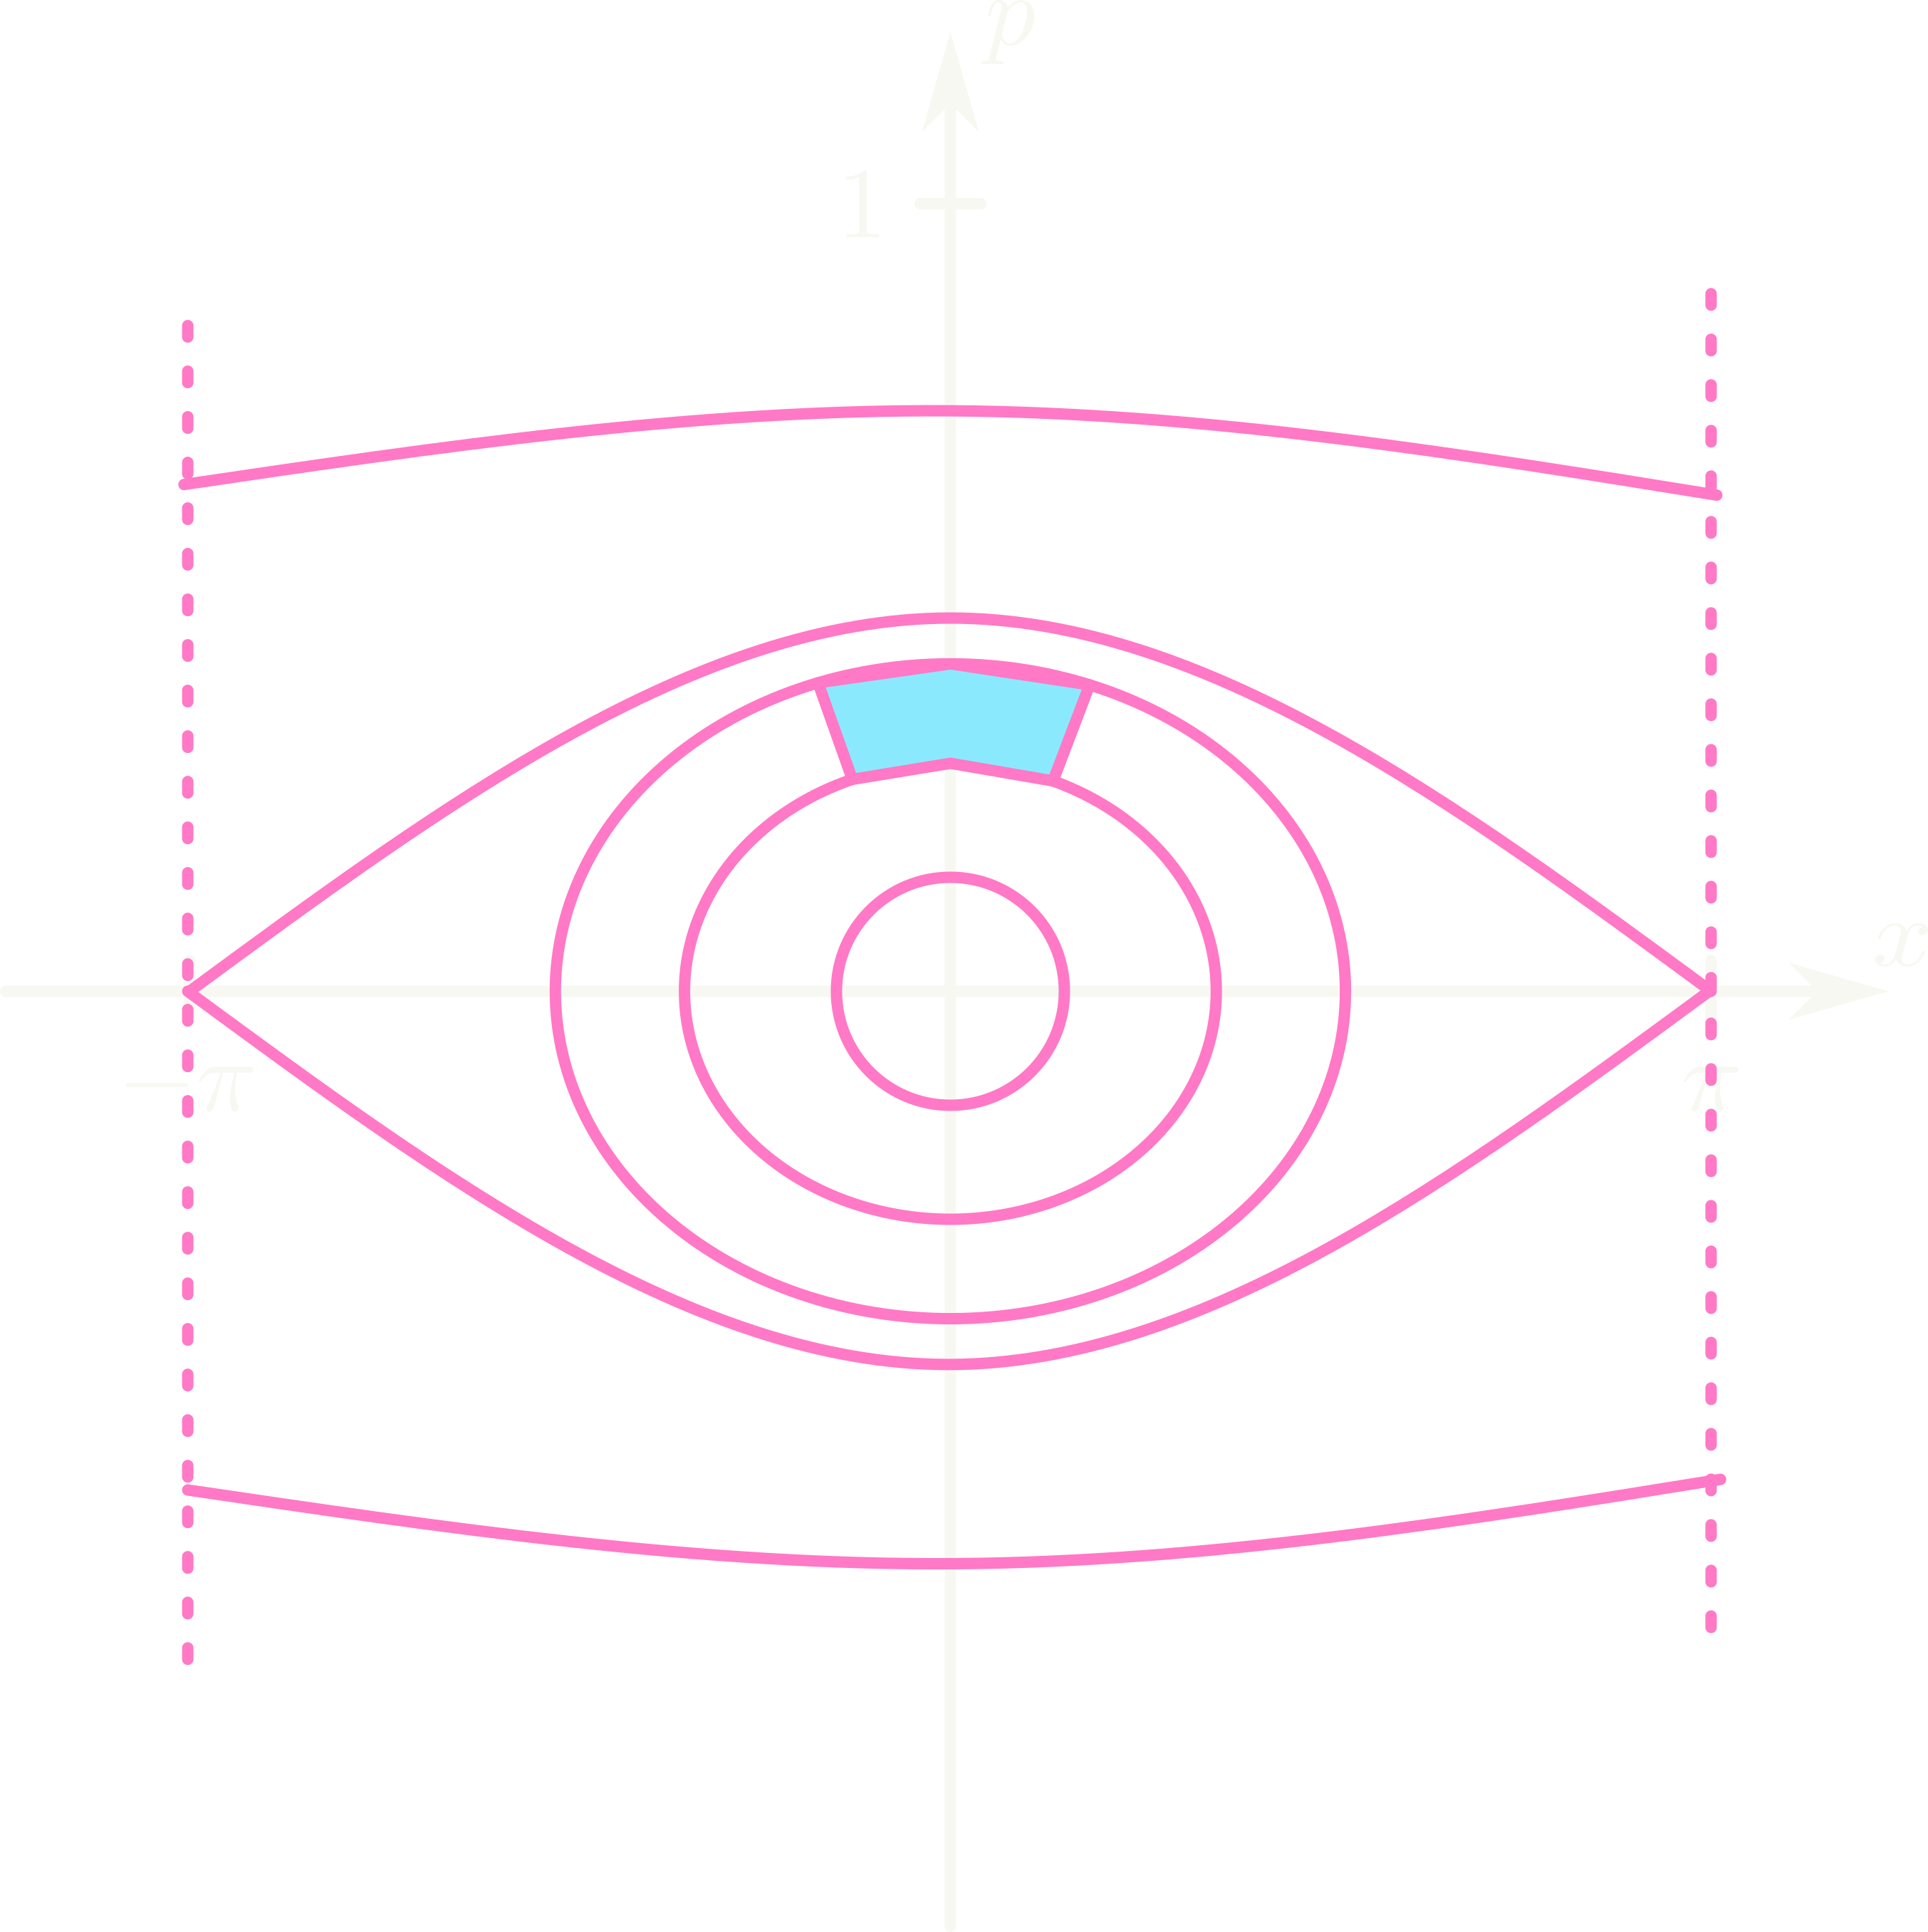
\includegraphics[width=0.5\textwidth]{images/phasespace.png}
    \caption{Phase Space for a Pendulum}
    \label{fig:phase_space}
\end{figure}
The volume of a region in the phase space which we can represent using the phase velocity
\begin{align*}
    \vb v_z = \dot{\vb z} = (\dot q, \dot p)
\end{align*}
The the volumet element is the flux of the phase velocity through the surface:
\begin{align*}
    \delta V = \oint_S \vb v_z \cdot \dd{\vb A}
\end{align*}
and from the divergence theorem:
\begin{align*}
    \oint_S \vb v_z \cdot \dd{\vb A} = \iiint_V \div{\vb v_z} \dd{V}
\end{align*}
And if the volume doesn't change with time then the divergence of the phase velocity is zero, i.e.,
\begin{align*}
    \div{\vb v_z} = 0
\end{align*}
Or
\begin{align*}
    \div{v_z} &= \pdv{\dot q}{q} + \pdv{\dot p}{p} = \pdv{v_x}{x} + \pdv{v_y}{y} = 0
\end{align*}
where
\begin{align*}
    \dot q &= \pdv{\mathcal{H}}{p} \quad \dot p = -\pdv{\mathcal{H}}{q}
\end{align*}
so we find that
\begin{align*}
    \div{v_z} = \pdv{\mathcal{H}}{q_i \partial p_i} - \pdv{\mathcal{H}}{p_i \partial q_i} = 0
\end{align*}
This tells us that the volume enclosed by a surface is conserved as it moves around in phase space.

\paragraph*{Example: Particles in a Volume}
We can consider a volume in phase space with density or distribution function $f$ where
\begin{align*}
    N &= \int f(x, p, t) \dd{V} \\
    \implies \dv{f}{t} &= 0 \qqtext{Vlasov Equation}
\end{align*}
The total derivative is zero, and in phase space the density of the volume would change. In
otherwords,
\begin{align*}
    \pdv{f}{t} + \dv{x}{t} \pdv{f}{x} + \dv{p}{t} \pdv{f}{p} &= 0 \\
    \pdv{f}{t} + v \pdv{f}{x} + F \pdv{f}{p} &=0 
\end{align*}
where $v$ is the velocity and $F$ is the force.
In branch of mathmatics, this describes Symplectic Geometry or Symplectic Manifolds.

\newpage
% Last week of classes
\section*{Nonlinear Dynamics}
\paragraph*{Last time:} Hamiltonian Mechanics; Poisson Brackets; Liouville's Theorem:
\begin{align*}
    [f, g] = 0
\end{align*}
Then $f, g$ are independent. In otherwords, $[f, \mathcal{H}] = 0$ means that $f$ is conserved.
\paragraph*{Phaase space Portrait:} 
\begin{align*}
    \begin{cases}
        \dot x = \frac{p}{m} \\
        \dot p = - \pdv{u}{x} = -u'
    \end{cases}
\end{align*}
\begin{figure}[ht]
    \centering
    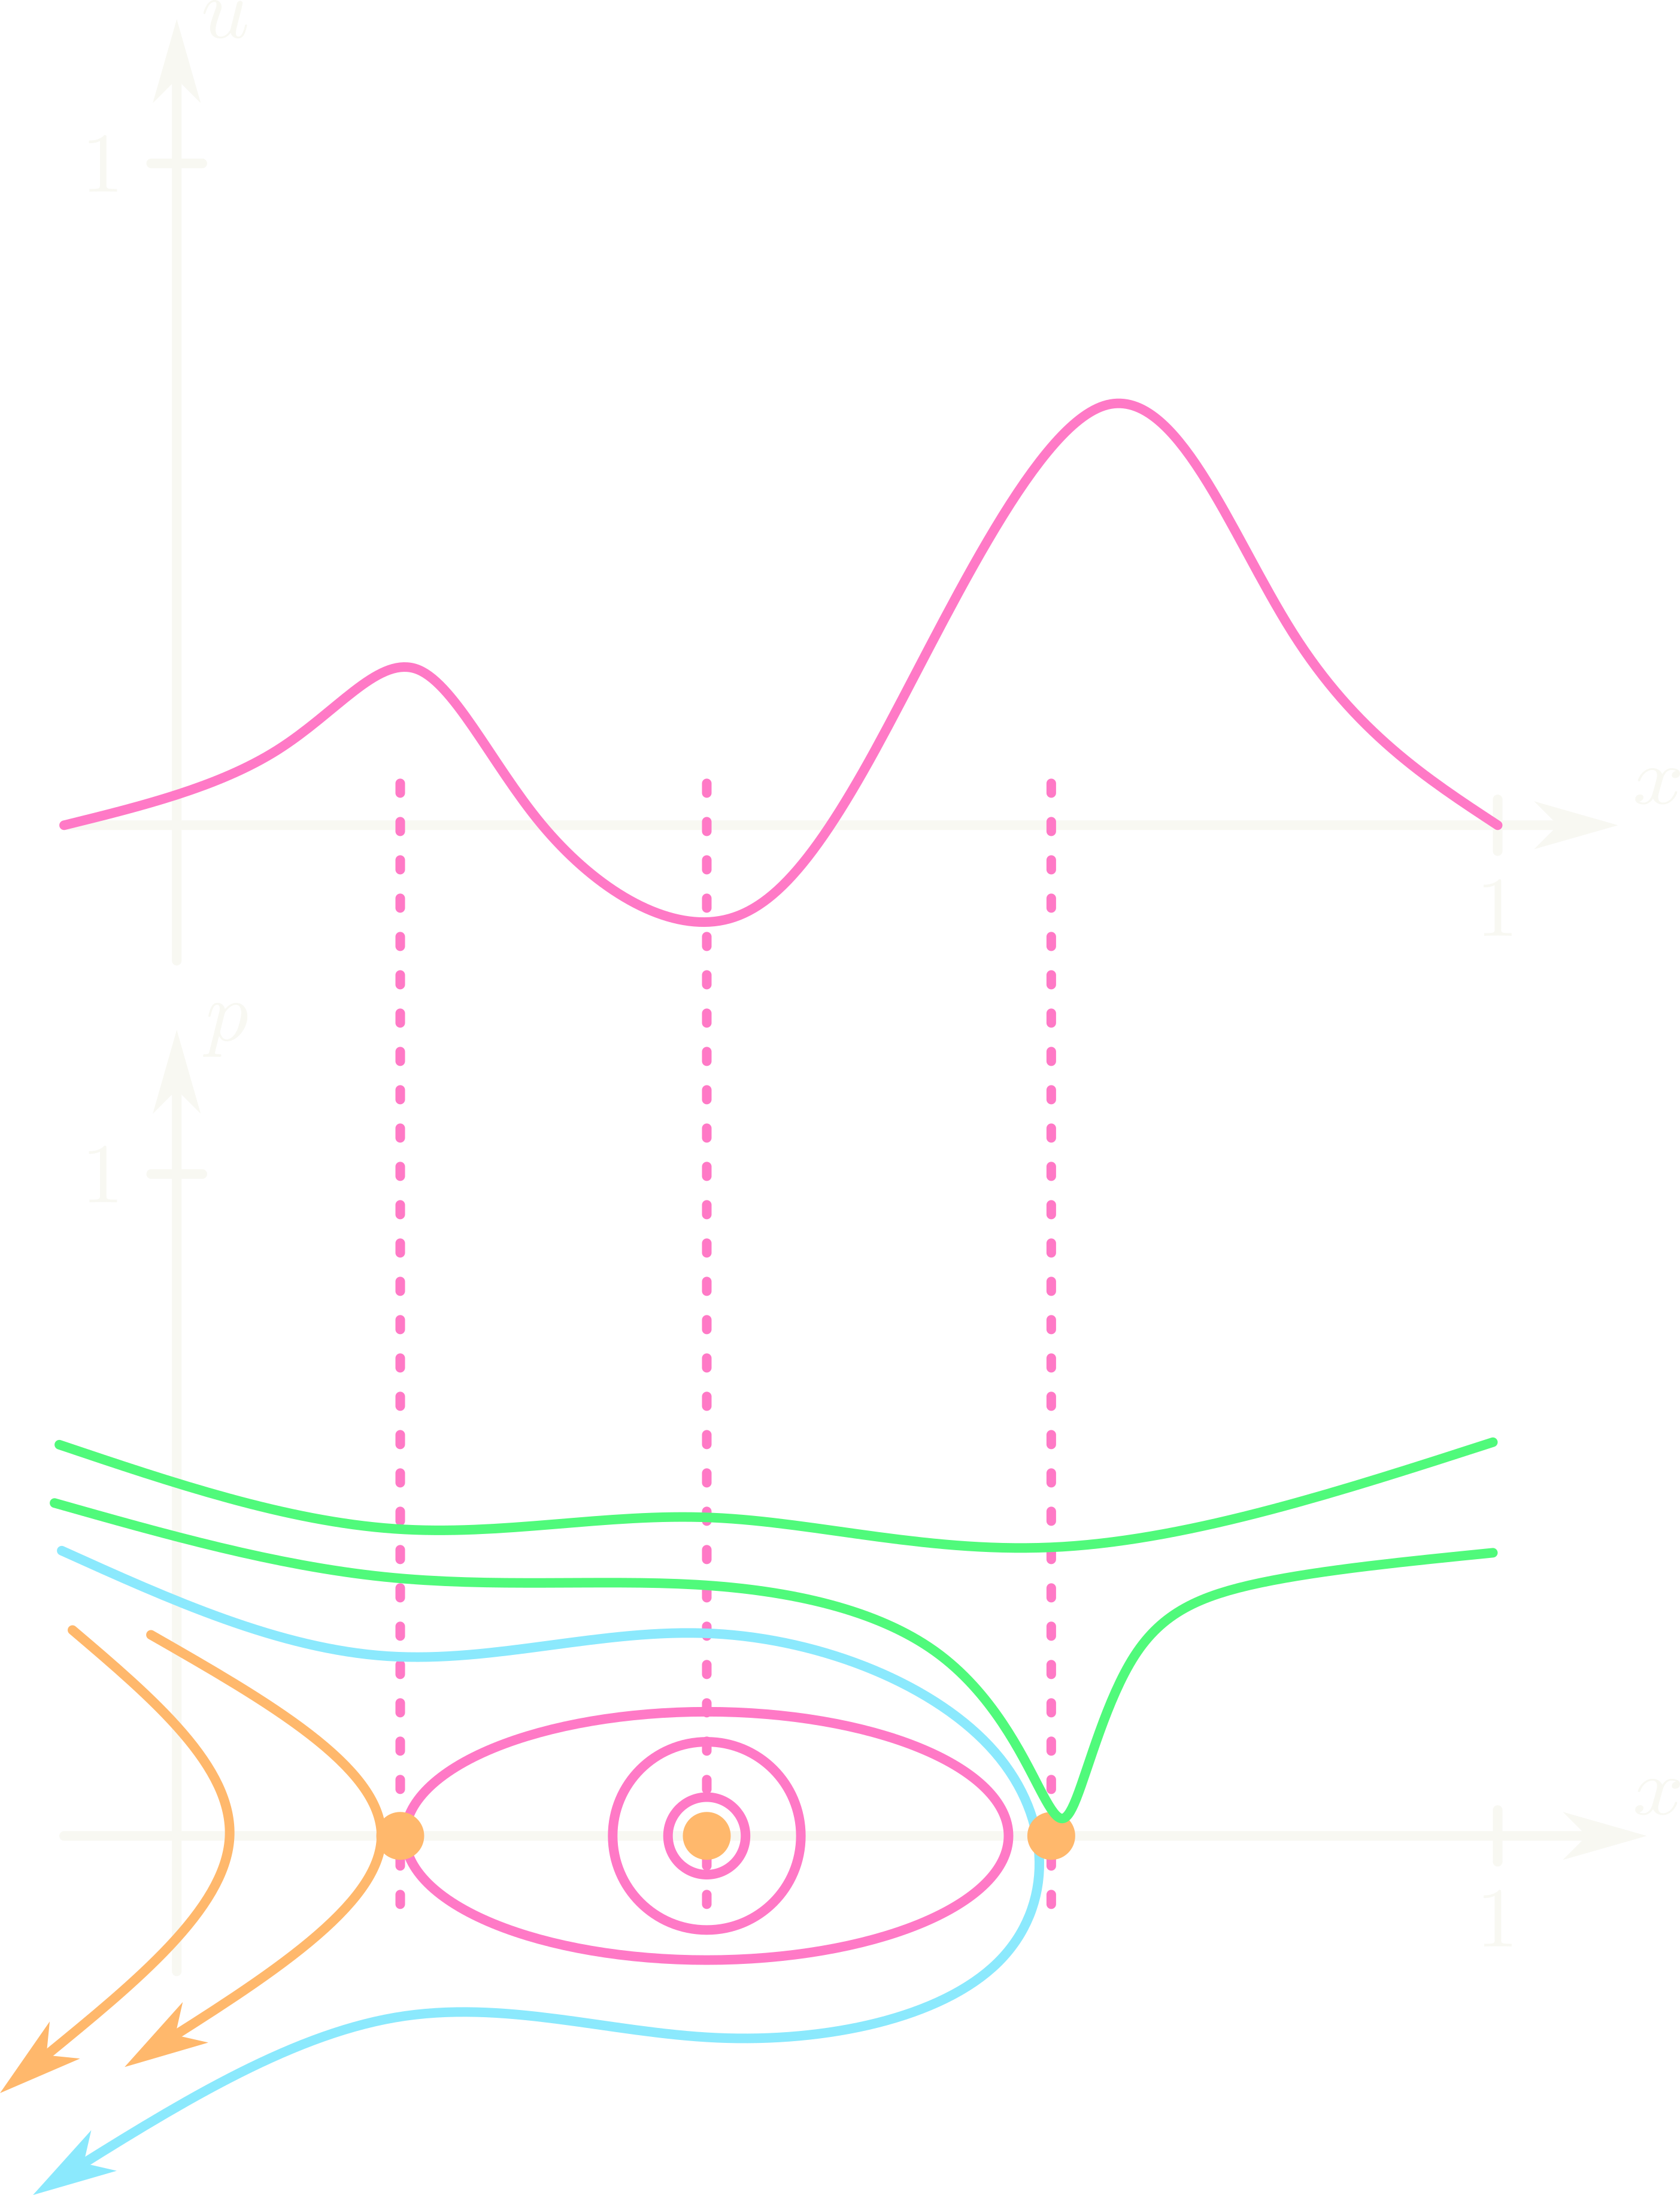
\includegraphics[width=0.5\textwidth]{phase_portrait.png}
    \caption{Phase Space Portrait}
\end{figure}

We can see at the center point, or equilibrium point, of the phase space portrait, we have a closed
path around it (pink orbit). The orbits from further away that do not go past the first
critical point circle back around as shown by the orange orbit, and if we start with higher
potential energy than the first  critical point(and not the third), it maintains a blue orbit. And
potentials larger than the third critical point will have a green orbit.

The critical points are given by 
\begin{align*}
    \dot x &= F(x,y) \\
    \dot y &= G(x,y)
\end{align*}
where $(x_0, y_0)$ is a critical point if $F(x_0, y_0) = G(x_0, y_0) = 0$.

\paragraph*{1D Motion} Under $u(x)$
\begin{align*}
    F = \frac{y}{m} \\
    G = -u'(x)
\end{align*}
and from the Jacobian
\begin{align*}
    J = \mqty(\pdv{F}{x} & \pdv{F}{y} \\ \pdv{G}{x} & \pdv{G}{y}) = \mqty(0 & \frac{1}{m} \\ -u''(x) & 0)
\end{align*}
Which has two eigenvalues $\lambda_1, \lambda_2$:
\begin{align*}
    \det J = \lambda_1 \lambda_2  = \frac{u''(x)}{m} \\
    \tr J = \lambda_1 + \lambda_2  = 0
\end{align*}
Since $u''(x) < 0$, both $\lambda_1, \lambda_2$ are real and opposite signs $\implies$ saddle point.

If $u''(x) > 0$, then $\lambda_1, \lambda_2 = \pm i v$ are purely imaginary $\implies$ center point.

\paragraph*{Brusselator}
\begin{align*}
    \dot x &= a - (1 + b) x + x^2 y \\
    \dot y &= bx - x^2 y
\end{align*}
Setting the two equations to zero, we find the critical points:
\begin{align*}
    a - (1 + b) x + x^2 y &= 0 \implies a - x = 0 \to x = a \\
    bx - x^2 y &= 0 \implies y = \frac{b}{a}
\end{align*}
So we have only one critical point at $(a, b/a)$. The Jacobian is
\begin{align*}
    J_{(a, b/a)} &= \mqty(b - 1 & a^2 \\ -b & -a^2) \\
    \tr J &= b - 1 - a^2 = b - (1 + a^2) = \lambda_1 + \lambda_2 \\
    \det J &= a^2 = \lambda_1 \lambda_2
\end{align*}
If $a,b$ are positive real numbers,
\begin{align*}
    b < 1 + a^2
\end{align*}
So the eigenvalues are both negative $\lambda_1, \lambda_2 < 0$, and a same sign
implies that every orbit spirals inward to the critical point (attracter). 

If $\lambda_1, \lambda_2 >0$ then the critical point is a repeller. Interestingly,
$b > 1 + a^2$ creates a limit cycle, where the critical poin is outside are repellers.
The two eigenvalues tell us the behavior along a particular direction, e.g., how the system behaves
near a critical point. 

\paragraph*{Rayleigh's equation}
\begin{align*}
    \ddot x &- \epsilon \dot x (1 - \dot x^2) + x = 0 \\
    \to \dot x &= y \\
    \dot y &= -x + \epsilon y(1 - y^2)
\end{align*}
where an obvious critical point is $(0,0)$. The path of the system for smaller $\epsilon$ will be
approaching a limit cycle around the critical point. Furthermore, for different $\epsilon$ values,
the shape of the limit cycle will change unintuitively.

\paragraph*{Lorenz System}
\begin{align*}
    \dot x &= \sigma(y - x) \\
    \dot y &= x(\rho - z) - y \\
    \dot z &= xy - \beta z
\end{align*}
For the $\sigma = 10, \rho = 28, \beta = 8/3$ values, the system has a chaotic behavior, aka the 
lorentz attractor.

\newpage
\subsection*{Order And Chaos}
What is chaos? Two points very close together in phase space $\delta \sim e^{\lambda t}$ will 
diverge exponentially so. The Lyapunov exponent $\lambda$ describes this rate of diveregence.
\begin{center}
    Chaos $\Leftrightarrow$ Sensitivity to initial condition 
    $\Leftrightarrow$ Loss of predictability 
    $\Leftrightarrow$ Butterfly Effect
\end{center}
The Butterfly effect is not a causal relationship (like the traditional metaphor).

\paragraph*{WHen is a system chaotic?}
\begin{itemize}
    \item Nonlinear
    \item \# of degrees of freedom $\geq 2 \geq$ 2D
    \item \# of conserved quanties $<$ \# of degrees of freedom. 
\end{itemize}
If not 3, then the system is ``integrable'' (in the sense of Liouville). The conserved quantities,
$[f, H]_p = 0$ and $[f_1, f_2] = 0$.
\paragraph*{Examples:}
\begin{itemize}
    \item A 1D system is always integrable, or not chaotic.
    \item A 2 body central force problem: We have 6 degrees of freedom, and 6 conserved quantities
    \begin{itemize}
        \item Center of Mass $R = (X, Y, Z)$
        \item Momentum $\vb P_R$
        \item Hamiltonian $H$
        \item $L_z$
        \item $L^2$
    \end{itemize}
    If we add a magnetic field $\vb B = B \vu z$ that interacts with the two bodies, the symmetry
    conserves $L_z$ but not $L^2$, so the system is chaotic.
    \item Rigid Body Motion: 3 dof (euler angles) and 3 conserved quantities
    \begin{itemize}
        \item $H, L_z, L^2$
    \end{itemize}
    means the system is not chaotic.
    \item The 3 body problem is chaotic.
\end{itemize} 
\paragraph*{Hierarchical Problem}
The Solar System is a predictable system because of the hierarchy of the masses relative to the sun:
\begin{align*}
    m_{\text{moon}} \ll m_{\text{earth}} \ll m_{\text{sun}}
\end{align*}
For example, the Hamiltonian of the Sun-Earth-Moon system would be approximately
\begin{align*}
    H = H_{E + S} + \delta H_{M}
\end{align*}
which makes the system ``nearly integrable''.

\paragraph*{Driven, Damped Pendulum}
From N2L
\begin{align*}
    m L \ddot \phi = - bL \dot\phi - mg \sin\phi + F(t) \\
    \to \ddot \phi + \frac{b}{m} \dot \phi + \frac{g}{L} \sin\phi = \frac{F(t)}{mL}
\end{align*}
which is similar to the driven damped oscillator, but now we have a non-linear sine term. 
Rewriting the equation with the familar damping coefficient ant natural frequency:
\begin{align*}
    2\beta = \frac{b}{m} \quad \omega_0^2 = \frac{g}{L}
\end{align*}
we get 
\begin{align*}
    \ddot\phi + 2\beta \dot\phi + \omega_0^2 \sin\phi = \frac{F}{mL} = \frac{F_0}{mL} \cos(\omega t)
\end{align*}
For small $\phi \ll 1$ we can approximate $\sin\phi \approx \phi$ and we have a solution which is
a linear combination of the homogenous(transient) and particular solutions:
\begin{align*}
    \phi(t) &= \phi_h(t) + \phi_p(t) \\
    &= e^{-\beta t} A_1 \cos(\omega_1 t) + A \cos(\omega t - \delta)
\end{align*}
and for $t \to \infty$
\begin{align*}
    \phi(t) = A \cos(\omega t - \delta)
\end{align*}
which is dependent on the driving force and the resonant frequency of the system. Using the next 
order term
\begin{align*}
    \sin\phi \approx \phi - \frac{\phi^3}{6}
\end{align*}
we get an equation of the form
\begin{align*}
    \ddot \phi + 2\beta \dot\phi + \omega_0 \qt(\phi - \frac{\phi^3}{6}) = \frac{F_0}{mL} \cos(\omega t) \\
    \to \ddot \phi + 2\beta \dot\phi + \omega_0^2 \phi = \frac{F_0}{mL} \cos(\omega t)
     + \frac{\omega_0^2}{6} A^3 \cos^3(\omega t - \delta)
\end{align*}
and using the trigonometric identity
\begin{align*}
    \cos^3x = \frac{1}{4}(\cos(3x) + 3 \cos x)
\end{align*}
so we have a form 
\begin{align*}
    \phi(t) = A \cos(\omega t - \delta) + B \cos(3\omega t - \delta)
\end{align*}

\newpage
\paragraph*{Final Lecture: DDP and Chaos}
The DDP is a nonlinear system but in one dimension\dots but in fact we have a dynamic
variable from the driving force:
\begin{align*}
    \dot\theta = \omega \implies \theta = \omega t \\
    \to 
    \ddot \phi + 2\beta \dot\phi + \omega_0^2 \sin\phi = \frac{F_0}{mL} \cos(\theta)
\end{align*}
So there are two degrees of freedom $\theta, \phi$. In addition, there are no conserved quantities
in the system. If the driving force depends on the force of gravity, i.e., 
\begin{align*}
    \gamma = \frac{F_0}{mg} \to \frac{F_0}{mL} \cos\theta = \gamma \omega_0^2 \cos\theta
\end{align*}
At small $\gamma$ we have a predictable motion where the period is the same as the driving force
frequency $P = 2\pi/\omega$. For larger $\gamma = 1.073$ we have a doubling of the period;
the position at each expected period drops slightly before going back to the original position.
At $\gamma = 1.081$ we have a period of 4. 
\paragraph*{Period Doubling Cascade}
At very large $\gamma$, the period will increase exponentially to infinity, and the system will fall
into ``chaos''. These bifucating points (the spliiting of the period), 
will bifurcate very quickly at a rate known as the Feigenbaum number $\delta$.


\end{document}